\begin{figure}[ht!]  % 'H' sugiere que la figura se coloque exactamente aquí
    \centering
    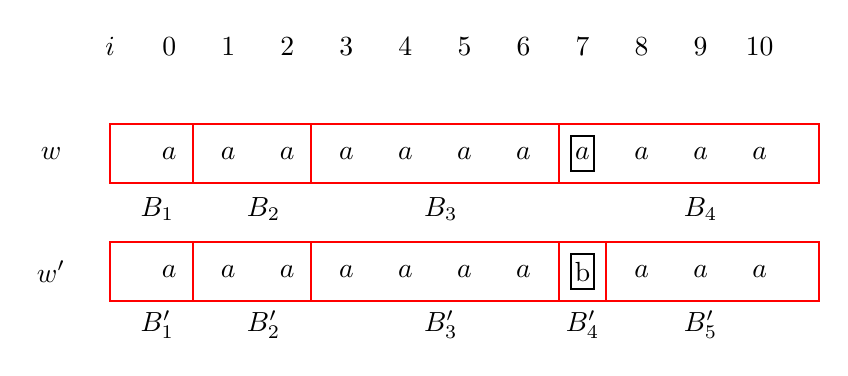
\begin{tikzpicture}[scale=1.5]
        % Rectángulo para w
        \draw (0,0) rectangle (6,0.5);
        \node at (-0.5, 0.25) {\(w\)};
        % Etiquetas dentro del rectángulo w
        \foreach \x/\char in {0.5/a, 1.0/a, 1.5/a, 2.0/a, 2.5/a, 3.0/a, 3.5/a, 4.0/a, 4.5/a, 5.0/a, 5.5/a}
            \node at (\x, 0.25) {\(\char\)};
        % \node at (5.7, 0.25) {\(...\)};

        \draw[draw=black, thick] (3.9,0.1) rectangle (4.1,0.4);
        % \draw[->, thick] (2.7,-0.5) -- (2.7,-0.2);
        % \node[align=center, above] at (4.0,0.6) {\(w[j]\)};
        
        % Rectángulo para w'
        \draw (0,-1) rectangle (6,-0.5);
        \node at (-0.5, -0.75) {\(w'\)};
        % Etiquetas dentro del rectángulo w' con un cambio de 'a' a 'b'
        \foreach \x in {0.5, 1.0, 1.5, 2.0, 2.5, 3.0, 3.5, 4.5, 5.0, 5.5}
            \node at (\x, -0.75) {\(a\)};

            
        % Cambiando un 'a' por un 'b'
        \node at (4.0, -0.75) {b};
        % \node at (5.7, -0.75) {\(...\)};

        \draw[draw=black, thick] (3.9,0.1) rectangle (4.1,0.4);
        \draw[draw=black, thick] (3.9,-0.9) rectangle (4.1,-0.6);
        % \draw[->, thick] (2.7,-0.5) -- (2.7,-0.2);
        % \node[align=center, above] at (4.0,-0.5) {\(w'[j]\)};
        \node[align=center, above] at (0.0,1) {\(i\)};
        \node[align=center, above] at (0.5,1) {\(0\)};
        \node[align=center, above] at (1.0,1) {\(1\)};
        \node[align=center, above] at (1.5,1) {\(2\)};
        \node[align=center, above] at (2.0,1) {\(3\)};
        \node[align=center, above] at (2.5,1) {\(4\)};
        \node[align=center, above] at (3.0,1) {\(5\)};
        \node[align=center, above] at (3.5,1) {\(6\)};
        \node[align=center, above] at (4.0,1) {\(7\)};
        \node[align=center, above] at (4.5,1) {\(8\)};
        \node[align=center, above] at (5.0,1) {\(9\)};
        \node[align=center, above] at (5.5,1) {\(10\)};


        \draw[draw=red, thick] (0,0) rectangle (0.7,0.5);
        \draw[draw=red, thick] (0.7,0) rectangle (1.7,0.5);
        \draw[draw=red, thick] (1.7,0) rectangle (3.8,0.5);
        \draw[draw=red, thick] (3.8,0) rectangle (6.0,0.5);
        \node[align=center, above] at (0.4,-0.4) {\(B_1\)};
        \node[align=center, above] at (1.3,-0.4) {\(B_2\)};
        \node[align=center, above] at (2.8,-0.4) {\(B_3\)};
        \node[align=center, above] at (5.0,-0.4) {\(B_4\)};
        
        
        \draw[draw=red, thick] (0,-1) rectangle (0.7,-0.5);
        \draw[draw=red, thick] (0.7,-1) rectangle (1.7,-0.5);
        \draw[draw=red, thick] (1.7,-1) rectangle (3.8,-0.5);
        \draw[draw=red, thick] (3.8,-1) rectangle (4.2,-0.5);
        \draw[draw=red, thick] (4.2,-1) rectangle (6.0,-0.5);
        \node[align=center, above] at (0.4,-1.4) {\(B'_1\)};
        \node[align=center, above] at (1.3,-1.4) {\(B'_2\)};
        \node[align=center, above] at (2.8,-1.4) {\(B'_3\)};
        \node[align=center, above] at (4.0,-1.4) {\(B'_4\)};
        \node[align=center, above] at (5.0,-1.4) {\(B'_5\)};

    \end{tikzpicture}
    \caption{Two inputs   $ w \sim w'$;  $w[j]=w[7]=a \neq w'[j]=w'[7]=b$; $n=11.$}
    \label{fig:two_input_changes}
\end{figure}